% !TeX root = CoPhy-Projekt.tex

%----------------------------------------------------------------%
%--------------------------GRUNDEINSTELLUNGEN--------------------%
%----------------------------------------------------------------%
\documentclass[oneside, ngerman, footinclude=off, captions=tableheading]{scrartcl}
%	'oneside'/'twoside': nicht zwischen linker und rechter Seite unterscheiden (alternativ twoside)
%	'twocolumn': wuerde 2 Spalten auf dem Blatt platzieren
%	'bibliography=totocnumbered': Normal nummeriertes Inhaltsverzeichnis (Kapitelnummer)
%	'listof=totocnumbered': Abbildungs- und Tabellenverzeichnis normal nummeriert (Kapitelnummer)
%	'ngerman' verwendet deutsch als Dokumentensprache (z.B. fuer Sirange)
%	'footinclude=off': Zaehlt Fusszeile zum Rand (vergroessert den Textbereich)
%	'captions=tableheading': Tabellenueberschriften explizit verwenden, erhoeht den Abstand zur Tabelle

\usepackage[ngerman]{babel}		%	Einstellen der Sprache
\usepackage[T1]{fontenc}		%	Wie wird Text ausgegeben, d.h. im PDF
\usepackage[utf8]{inputenc}		%	Welche Zeichen 'versteht' LaTeX bei der Eingabe?
\usepackage{lmodern}			%	Laedt Schriften, die geglaettet sind
\usepackage{blindtext}			%	Beispieltext, zum Testen geeignet

%----------------------------------------------------------------%
%--------------------------ABSTÄNDE------------------------------%
%----------------------------------------------------------------%
%\usepackage[onehalfspacing]{setspace}				%	Für Zeilenabstaende: 'singlespacing' (einfach), 'onehalfspacing' (1.5-fach), 'doublespacing' (2fach)
%\setlength{\parindent}{0cm}						%	Laengenangabe für die Einrueckung der ersten Zeile eines neuen Absatzes.
%\setlength{\parskip}{6pt plus 3pt minus 3pt}		%	Laengenangabe für den Abstand zwischen zwei Absaetzen.
%	Wenn diese beiden Befehle nicht kommentiert sind, wird ein Absatz nicht eingezogen sondern es gibt einen Abstand

% kleinere Abstände über und unter Gleichungen
\usepackage{setspace}\onehalfspacing
\AtBeginDocument{%
  \addtolength\abovedisplayskip{-0.2\baselineskip}
  \addtolength\belowdisplayskip{-0.2\baselineskip}
}

%----------------------------------------------------------------%
%--------------------------MATHE---------------------------------%
%----------------------------------------------------------------%
\usepackage[]{mathtools}							%	Erweiterung von AMSMath, laedt automatisch AMSMath - für viele Mathe-Werkzeuge, 'fleqn' als Option ist für Mathe linksbuendig
\usepackage{amsfonts}								%	Für eine Vielzahl an mathematischen Symbolen
\usepackage{nicefrac}

%----------------------------------------------------------------%
%--------------------------KOPF- UND FUSSZEILEN------------------%
%----------------------------------------------------------------%
\usepackage[automark,headsepline=.4pt]{scrlayer-scrpage}
\pagestyle{scrheadings}
\setkomafont{pageheadfoot}{\normalfont\bfseries}	%	Normale Schriftart und Fett für den Seitenkopf
\addtokomafont{pagenumber}{\normalfont\bfseries}	%	Normale Schriftart und Fett für die Seitenzahl
\clearpairofpagestyles								%	Löscht die Seitenkopf- und Seitenzahlen
\ohead{\thepage}									%	Rechter Seitenkopf mit Seitenzahl
\ihead{\headmark}									%	Linker Seitenkopf mit section
\ofoot[]{\empty}									%	Leere Fußzeile, ungerade Seiten
%	Definert man oben in der documentclass 'twoside', so wird zwischen geraden und ungeraden Seiten unterschieden (NUR DANN!)

%----------------------------------------------------------------%
%--------------------------BILDER--------------------------------%
%----------------------------------------------------------------%
\usepackage{graphicx}									%	Um Bilder einbinden zu koennen 
\usepackage[dvipsnames,svgnames,table]{xcolor}			%	Farben verwenden, Versch. Farbdefinitionen, Farben in Tabellen (-Reihen, -Spalten)
\usepackage{pdfpages}									%	pdfs importieren
\definecolor{Seeblau100}{RGB}{0,169,224}				%	Uni-Farben, z.B. fuer Tabellen
\definecolor{Seeblau65}{RGB}{89,199,254}
\definecolor{Seeblau35}{RGB}{165,224,254}
\definecolor{Seeblau20}{RGB}{203,237,254}
\definecolor{Seegrau60}{RGB}{102,102,102}
\definecolor{Seegrau40}{RGB}{153,153,153}
\definecolor{Seegrau20}{RGB}{204,204,204}
\definecolor{Seegrau10}{RGB}{230,230,230}

%----------------------------------------------------------------%
%--------------------------POSITIONIERUNG------------------------%
%----------------------------------------------------------------%
\usepackage{float}

%----------------------------------------------------------------%
%--------------------------LISTEN--------------------------------%
%----------------------------------------------------------------%
\usepackage{enumitem}							%	Um Listen / Aufzaehlungen leichter zu modifizieren
%\setlist{noitemsep}							%	Verringert den Abstand in Aufzaehlungen

%----------------------------------------------------------------%
%--------TABELLEN-/BILDUNTERSCHRIFTEN und NUMMERIERUNG-----------%
%----------------------------------------------------------------%
\addtokomafont{captionlabel}{\bfseries}			%	Abbildung X.Y wir fett geschrieben
\setcapindent{2em}								%	2. Zeile teilweise haengend und eingezogen. Wenn ganz haengend gewuenscht, auskommentieren


%----------------------------------------------------------------%
%--------------------------LITERATURVERZEICHNIS------------------%
%----------------------------------------------------------------%
\usepackage[german]{babelbib}					%	Bereitstellung des deutschen Layouts fuer die Bibliography
\bibliographystyle{babalpha}

%----------------------------------------------------------------%
%--------------------------SIUNITX-------------------------------%
%----------------------------------------------------------------%
\usepackage[]{siunitx}
\DeclareSIUnit\octave{oct}
\DeclareSIUnit\Hz{Hz}
\sisetup{locale = DE}							%	Automatische Einstellung der Ausgabe für bestimmte Regionen (UK, US, DE, FR, ZA)
\sisetup{separate-uncertainty = false
}

%----------------------------------------------------------------%
%--------------------------URLs / REFs---------------------------%
%----------------------------------------------------------------%
\usepackage[hidelinks]{hyperref}				%	Erweiterte Referenzierung ('hidelinks' verhindert Linien um Links)

%----------------------------------------------------------------%
%--------------------------EIGENE BEFEHLE------------------------%
%----------------------------------------------------------------%

\usepackage{todonotes}
\usepackage{wrapfig}
\setlength{\intextsep}{0pt}%
\usepackage{multicol}

\usepackage{listings}
\usepackage{xcolor}

\definecolor{codegreen}{rgb}{0,0.6,0}
\definecolor{codegray}{rgb}{0.5,0.5,0.5}
\definecolor{codepurple}{rgb}{0.58,0,0.82}
\definecolor{backcolour}{rgb}{0.95,0.95,0.92}

\lstdefinestyle{mystyle}{  
    commentstyle=\color{codegreen},
    keywordstyle=\color{magenta},
    numberstyle=\tiny\color{codegray},
    stringstyle=\color{codepurple},
    basicstyle=\ttfamily\footnotesize,
    breakatwhitespace=false,         
    breaklines=true,                 
    captionpos=t,                    
    keepspaces=true,                 
    numbers=left,                    
    numbersep=5pt,                  
    showspaces=false,                
    showstringspaces=false,
    showtabs=false,                  
    tabsize=2
}


\lstset{style=mystyle}


\begin{document}

\title{Computerphysik I: Swing-by Manöver}
\author{Aurel Müller-Schoenau, Leon Oleschko und Moritz Schröer}
\maketitle

\begin{abstract}	
\end{abstract}

\section{Einleitung}
Beim Swing-By geht es darum, einen Satelliten gezielt an einem Himmelsobjekt vorbeifliegen zu lassen, damit die wirkende Gravitation den Satelliten auf einen gewünschten Orbit bringt. Dadurch lässt sich der sonst zur Beschleunigung benötigte Treibstoff sparen.\\
In diesem Bericht geht es um eine historische Raumfahrtmission der ESA, es handelt sich um die Ulysses-Raumfahrtmission. Bei dieser wurde nur ein Swing-by, nämlich am Planeten Jupiter, durchgeführt und die Daten zur Flugbahn sind verfügbar\footnote{\url{https://www.cosmos.esa.int/web/ulysses/mission-trajectory}}. Ziel ist es, mithilfe einer Simulation anhand der Shooting-Methode herauszufinden, wie der Satellit von der Erde aus ins All geschickt werden muss, um einen Swing-By auf den entsprechenden Orbit zu erreichen, und dann den errechneten Orbit mit den historischen Daten zu vergleichen.

\section{Trajektorie}
\begin{figure}[h!]
	\centering
	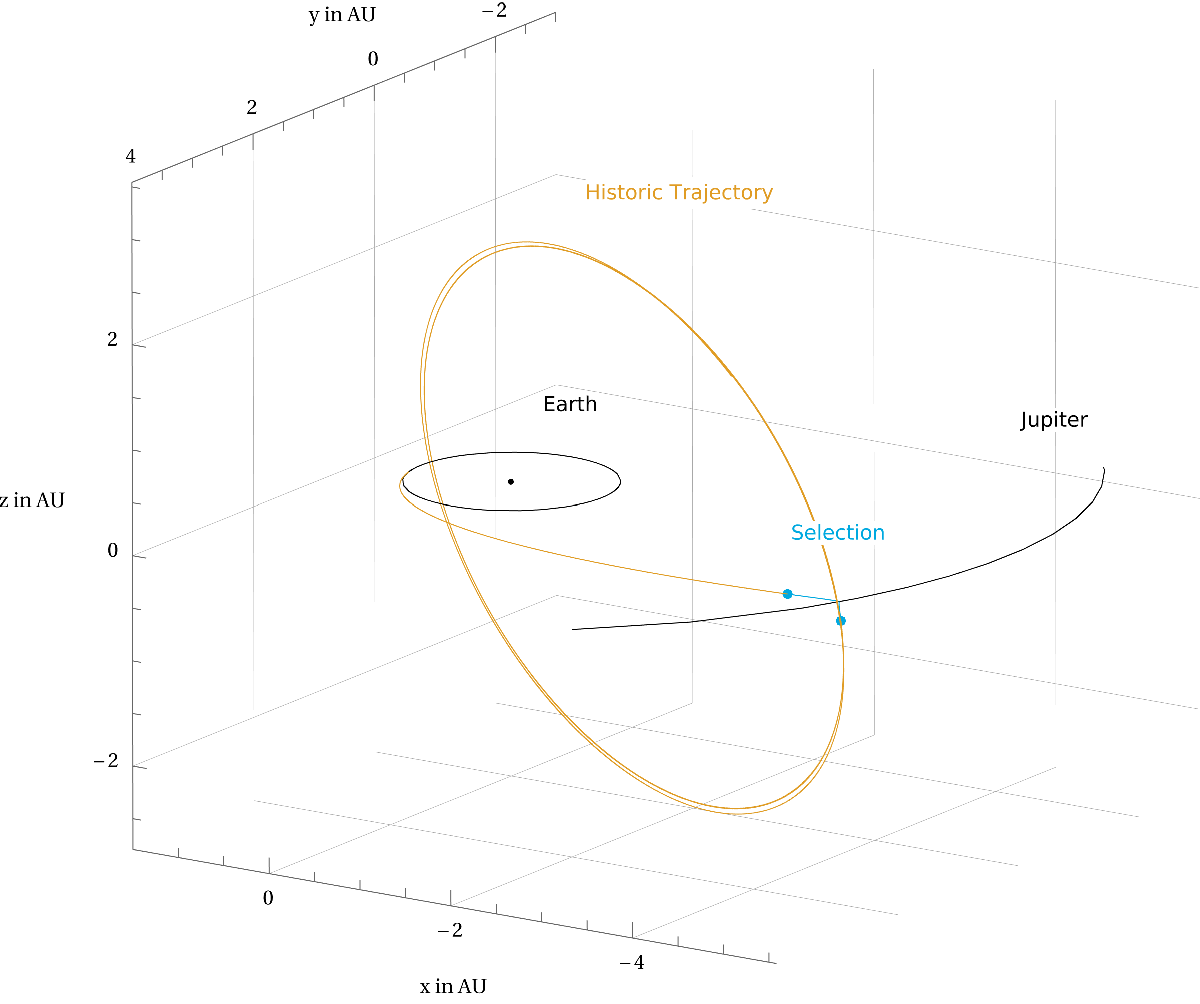
\includegraphics{img/trajectory.pdf}
	\caption{Abbildung der historischen Trajektorie, der simulierten Flugbahn und der relevanten Himmelskörpern}
	\label{fig:trajectory}
\end{figure}

Um die Flugbahn zu simulieren, muss die wirkende Gravitationskraft berechnet werden.
Zu Vereinfachung werden nur die Sonne, die Erde und der Jupiter berücksichtigt, weil der Satellit an keinem anderen Planeten nahe vorbeiflog.
Die Planeten-Daten wurden aus Mathematica\footnote{Wolfram Research, Inc., Wolfram|Alpha Notebook Edition, Champaign, IL (2022).} in gebräuchlicher Auflösung exportiert, um die Datenmenge zu reduzieren.
Da die Koordinaten nur tageweise vorliegen, werden sie in der Simulation linear über den Tag interpoliert.
In Abbildung \ref{fig:trajectory} sind die Positionen der Planeten, die Historische Trajektorie und ein simulierte Flugbahn dargestellt.

Für die Simulation wurde eine Dauer von 2800 Tagen betrachtet, wobei der Satellit historisch ungefähr 474 Tage für den Transfer zum Jupiter benötigte, und in der restlichen Zeit etwa einen vollständigen Orbit nach dem Swing-By durchlief.
Jeder dieser Tage wurde in 1000 Zeitschritte aufgeteilt, da bei mehr Schritten sich die Ergebnisse nicht mehr verändert haben.
Für jeden dieser Schritte wurde ein Leap-Frog-Schritt durchgeführt, um die Position und Geschwindigkeit des Satelliten zu berechnen. Dabei wurden die Positionen der Himmelskörper als vom Satelliten unbeeinflusst angenommen.


\begin{figure}[h!]
	\centering
	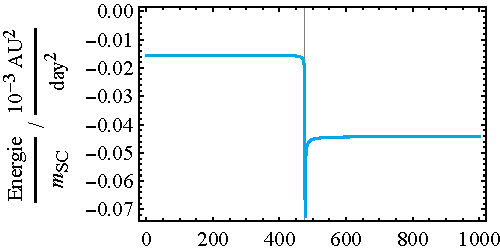
\includegraphics{img/energy.pdf}
	\caption{Energieänderung während des Swing-by Manövers}
\end{figure}


\section{Fehlerfunktionen}
\begin{figure}[h!]
	\centering
	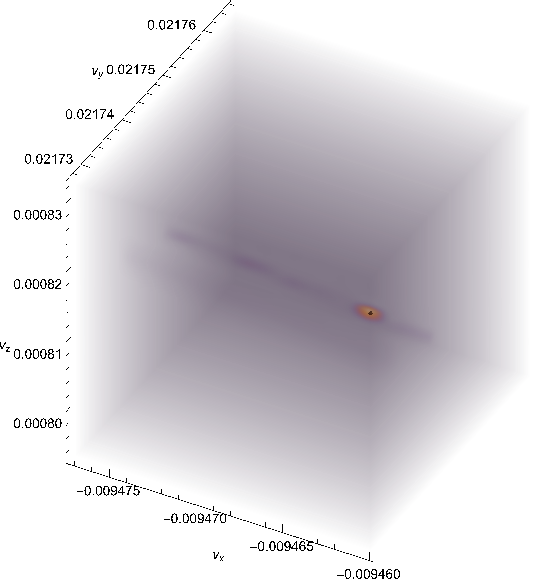
\includegraphics{img/gridSearch.pdf}
\end{figure}

Damit ein gewünschter Orbit erreicht werden kann, muss zunächst definiert werden, wie dieser aussehen soll. Der Starpunkt des Satelliten liegt natürlich auf der Erde. Den genauen Endzustand kennen wir im Fall der historischen Raumfahrtmission, ansonsten bleibt nur übrig, den gewünschten Zielorbit auf andere Weise zu definieren. In beiden Fällen handelt es sich um ein Randwertproblem, welches sich mithilfe der Shooting-Methode lösen lässt.\\
Dazu definieren wir eine Fehlerfunktion, die genau dann zu null wird, wenn der Satellit sich am Ende der Simulationszeit auf dem gewünschten Kurs befindet.
Um den Satelliten in unserer Simulation auf den finalen Orbit des Ulysses-Satelliten zu schicken, haben wir verschiedene Fehlerfunktionen ausprobiert.


\subsection{Vergleich der Endgeschwindigkeit und des Ortes}

Um einen Orbit zu erhalten, der dem historischen ähnelt, wurde zunächst \textit{zu einem festen Zeitpunkt} nach dem Swing-By der \textit{Ort und die Geschwindigkeit} des Satelliten mit den historischen Daten verglichen. Da diese keine Geschwindigkeitsinformationen enthalten, wurde dafür die mittlere Geschwindigkeit des Tages angenommen. \\
Der Ort allein als Vergleichswert reichte nicht aus, da das Programm sonst eine Abkürzungslösung fand, bei der der Satellit an der (im Vergleich zu den historischen Daten) entgegengesetzten Seite des Jupiter vorbeiflog, dadurch jedoch beim Swing-By in die falsche Richtung, und somit nicht auf den gewünschten Orbit abgelenkt wurde.

\subsection{Mehre Endpunkte zu festen Zeiten}

Eine andere Methode ist der Vergleich der \textit{Ort}skoordinaten nach dem Swing-By \textit{zu mehreren Zeitpunkten}, dafür aber \textit{ohne Vergleich der Geschwindigkeiten}. Der Zielorbit wird nun also durch eine Reihe an zu erreichenden Wegpunkten definiert, die zu bestimmter Zeit zu erreichen sind.

\subsection{Integral des Ort-Fehler-Quadrates}




\subsection{Vergleich von Zielpunkten bei nächster Zeit}

Um die Tatsache, dass in der Realität bei der Planung eines Swing-By-Manövers wahrscheinlich keine passenden Daten vorlägen, nicht völlig außer Acht zu lassen, wurden bei der dritten Fehlerfunktion einige Punkte auf dem Wunsch-Orbit ausgewählt - in unserem Fall genau solche, die in den historischen Daten vorlagen, aber es hätten beliebige Punkte sein können. Und dann wurde beim Berechnen der Trajektorie bei jedem Zeitschritt der aktuelle Abstand zu jedem der ausgewählten Punkte gemessen. Der Wert wurde mit einem gespeicherten Wert verglichen, und dieser überschrieben, falls der aktuelle Wert kleiner war. So wurde zu jedem der ausgewählten Punkte der nächstgelegene Punkt der aktuellen Trajektorie gefunden.\\
Bei dieser Methode muss also der Zeitpunkt des Manövers nicht im Voraus bekannt sein, jedoch besteht die Möglichkeit, dass ein korrekter Orbit nicht erkannt wird, wenn die ausgewählten Punkte des gewünschten Orbits gerade zwischen denen des berechneten Orbits liegen. Solange die Zeitschritte klein genug sind, wird dann aber der Fehler immernoch sehr klein. Es wurde deshalb \textit{bei jedem Sub-Step}, also pro tausendstel Tag, der Abstand verglichen.






\section{Optimierung}
Die Shooting-Methode besteht nun darin, die Fehlerfunktion für einen gegebenen Orbit auszuwerten, und ausgehend davon den Orbit in irgendeiner Weise anzupassen, um schließlich die Nullstelle der Fehlerfunktion zu finden.
Als Optimierungsparameter wurde die Anfangsgeschwindigkeit gewählt, da diese nur 3 Dimensionen hat und somit leichter zu optimieren ist, als z.B. der Transferorbit.
Als initialer Wert wurde die echte gemessene Geschwindigkeit verwendet. Wichtig war vor allem, eine Anfangsgeschwindigkeit zu wählen, für welche der Satellit möglichst nahe am Jupiter vorbeifliegt, um die Laufzeit des Suchalgorithmus zu verringern. \\
Die Daten liegen aber in Form von Kooridinaten in einem sphärischen heliozentrischen Koordinatensystem vor und haben eine Auflösung von $0.01\text{°}$.
Daraus lässt sich eine Unsicherheit der Position von $4\;\text{AU}\cdot\sin 0.01\text{°}\approx 7\cdot 10^{-4}\;\text{AU}$ und daraus eine Unsicherheit der Geschwindigkeit von $\sqrt{2}\cdot 7\cdot 10^{-4} \approx 10^{-3}\;\text{AU/day}$ abschätzen.
Solche Unsicherheit ist viel zu groß für die nötige Genauigkeit von $10^{-6}$ bis $10^{-8}\;\text{AU/day}$, denn so viele Stellen muss der Suchalgorithmus optimieren, um die Nullstelle der Fehlerfunktion möglichst genau zu finden. Eine sehr kleine Änderung der Startgeschwindigkeit kann bereits zu einem völlig anderen Orbit führen. Dies dämpft die Erwartungen an die Ergebnisse.\\
Zur Nullstellensuche wurden verschiedene Verfahren ausprobiert.

\subsection{Newton-Verfahren}

Die Nullstelle einer stetig differenzierbaren Funktion lässt sich mithilfe des Newton-Verfahrens finden. Dabei wird die Funktion lokal linear durch ihre Ableitung angenähert. Ist die Determinante der Ableitung ungleich Null, so lässt sich das entsprechende Gleichungssystem für jedes gewünschte Ergebnis eindeutig lösen. Die Nullstelle der Taylor-Entwicklung bis zur ersten Ordnung an einem beliebigen Startpunkt wird auf diese Weise bestimmt, und die Lösung wird als neuer Startwert für die nächste Iteration desselben Vorgehens verwendet. \\
Das Newton-Verfahren konvergiert unter bestimmten Bedingungen (die unsere Fehlerfunktionen erfüllen) lokal quadratisch gegen eine Nullstelle der untersuchten Funktion (ohne Beweis).

\subsection{Newton-Hesse-Verfahren}



\subsection{Gradienten-Verfahren}

\section{Diskussion der Ergebnisse und Probleme}

Bei den Berechnungen der Trajektorie konnten mit keiner der benutzen Methoden eine exakte Reproduktion der historischen Daten erreicht werden. Es gibt mehrere mögliche Fehlerquellen, die die Genauigkeit der Berechnungen einschränken. Eines der Probleme, welches alle bei diesem Projekt implementierten numerischen Optimierungsverfahren haben ist, dass diese nur lokal konvergent sind. Das entscheidende  Problem der lokalen Konvergenz kann dabei mittels der bei dem Projekt implementierten \glqq Grid-Search-Methode\grqq\, gezeigt werden. Bei der \glqq Grid-Search-Methode\grqq\, werden die Werte der verwendeten Fehlerfunktionen für ein feines Gitter von Anfangsgeschwindigkeiten berechnet. Das Gitter von Anfangsgeschwindigkeiten umfasst dabei einen gewissen Geschwindigkeitsbereich welcher sich um die gesuchte Anfagsgeschwindigkeit erstreckt. Dabei hat sich gezeigt, dass die untersuchten Fehlerfunktionen mehrere lokale Minima im Bereich der gesuchten Lösung besitzen, welche nur sehr geringe Abstände zueinander haben. Das hat zur Folge, dass die lokal konvergenten Optimierungsverfahren, nicht immer gegen die gesuchte Lösung konvergieren. Besonders beim Newton-Verfahren zur Suche von Minima (in Kapitel 4.2 beschrieben) hat sich gezeigt, dass dieses aufgrund der vielen lokalen Minima, für diese Art von Problemstellung eher ungeeingnet ist.

\section{Fazit}


\end{document}

